\RequirePackage{filecontents}

\documentclass[conference]{IEEEtran}
% If the IEEEtran.cls has not been installed into the LaTeX system files,
% manually specify the path to it.  e.g.
% \documentclass[conference]{./IEEEtran}

% Add and required packages here
\usepackage{graphicx,times,amsmath}

% Correct bad hyphenation here
\hyphenation{op-tical net-works semi-conduc-tor IEEEtran}

% To create the author's affliation portion using \thanks
\IEEEoverridecommandlockouts

\textwidth 178mm
\textheight 239mm
\oddsidemargin -7mm
\evensidemargin -7mm
\topmargin -6mm
\columnsep 5mm

%\setlength{\parskip}{0.5em}

\begin{document}

% Project title: keep the \ \\ \LARGE\bf in it to leave enough margin.
\title{\ \\ \LARGE\bf Monte-Carlo Tree Search for Robocode}

\author{Jacob Grooss (jcgr@itu.dk), Jakob Melnyk (jmel@itu.dk)}

% Uncomment out the following line for invited papers
%\specialpapernotice{(Invited Paper)}

% Make the title area
\maketitle

\begin{abstract}
Monte-Carlo Tree Search (MCTS) generally performs well in games where it is able to correctly simulate game states and adversarial behaviour. The goal of this paper is to explore whether MCTS is capable of performing well in partially observable games where there is no single best strategy for the adversary to use.

We compare four different versions of an MCTS controller for the game Robocode by matching them up against simple controllers included with the game. Our best controller performed quite poorly against the included controllers. Our results suggest that regular MCTS is unlikely to perform well in these kinds of environments, however a number of changes to the algorithm would likely result in a vast improvement of performance

\end{abstract}

\section{Introduction}
\label{01}
\PARstart{M}{o}st games attempt to engage the player by presenting a number of challenges for the player to overcome. Sometimes these challenges consist of precision, timing, execution speed and reaction time, while in other cases the challenge consists of making a strategic choice. When a player must make a 


What problem are you trying to solve? Why is this important?\cite{FearAI}


\section{Background}
\label{02}
Most games attempt to engage the player by presenting a number of challenges for the player to overcome. Sometimes these challenges consist of precision, timing, execution speed and reaction time, while in other cases the challenge consists of making a strategic choice. When making these strategic choices, a player must consider not only the present state of the game, but also the actions taken by the adversary (either another player, an artificial intelligence or the game itself). 

\subsection{Monte-Carlo Tree Search}
\label{02_MCTS}

Monte-Carlo Tree Search (MCTS)\cite{browne2012survey} is a searching algorithm that is based on the Monte Carlo method, which dates back to the 1940s. The idea behind the MCTS algorithm was explored in the 1980s and various implementations were written in the following years. It was not, however, until 2006 where a breakthough was made, which made AIs able to utilize MCTS to play games that had been considered too challenging until then, such as Go\cite{gelly2011monte}\cite{chaslot2010monte}.

MCTS is, as the name implies, a tree search algorithm. Unlike other tree searches, it is a highly selective, best-first search that is able to figure out which parts of the search space that are the most promising and thus focus on that.

In order to determine the most promising part of the search space, MCTS runs a lot of \textit{playouts}. \textit{Playouts} are simulations of playing the game until an end condition is reached, with each move being chosen at random. The score of the game state at the end is based on the UCT and is used to update the weights of the tree in such a way that better nodes are more likely to be explored further.

The better the heuristic is at determining the value of a gamestate, the better MCTS will fare. An example of this is to factor in how many lives Pac-Man has left at an end state instead of only evaluating at the score.

% Discuss heuristic, general usefulness

\subsection{MCTS in Partially Observable Games}

MCTS works on the premise of information. The more it knows about what is going on, the better it performs. This means that in fully observable games, such as chess or Pac-Man, where it has access to all information about a game state, MCTS will perform well. Based on this fact, it is sensible to assume that MCTS will not perform as well in partially observable games. 

Imagine a version of chess where you do not know the position of your opponent's pawns until you try to move a piece to their position or they are within one square of any of your pieces. In such a game, MCTS would not be able to properly evaluate various game states, as it does not have the necessary information to do so. It can assume that the opponent plays in a certain way and evaluate the search space based on that, but it will not be accurate at all times.

That a game is only partially observable does not mean that MCTS will not work. It simply means that algorithm will have to take into account that there are things it does not know and that it therefore must attempt to figure these things out. 

Research indicates that is is possible to write MCTS implementations that works in a partially observable environment. The research has been done on very simple games (phantom tic-tac-toe)\cite{auger2011multiple} and on systems where it is possible to build a history of previously encountered states and run statistics on that\cite{silver2010monte}\cite{thrun1999monte}. While they are not developed enough to work with most partially observable games, it does prove that MCTS can be adapted to such games, given the right methods.

% Mention other research, discuss potential problems with inaccurate evaluation of states



%Has this been done before? 
%How? 
%If not, what’s the closest related research? (Both using similar approaches and other algorithms.) 
%What’s novel with your research?


\section{Game Mechanics}
\label{03}

The game we use is called "Robocode"\cite{robocode}. It is a programing game where the players program robots to battle other players' robots. 

Fights between robots take place on a battlefield (see figure \ref{figure-RobocodeBattle01}), which is represented as a Cartesian coordinate system, with (0, 0) being in the lower left corner. Distances are measured in pixels and directions are measured in degrees, where north is 0 degrees, east is 90 degrees, south is 180 degrees and west is 270 degrees. Robots decide on what action they want to take and all robots' actions are then carried out simultaneously.

\begin{figure}[htp]
\centerline{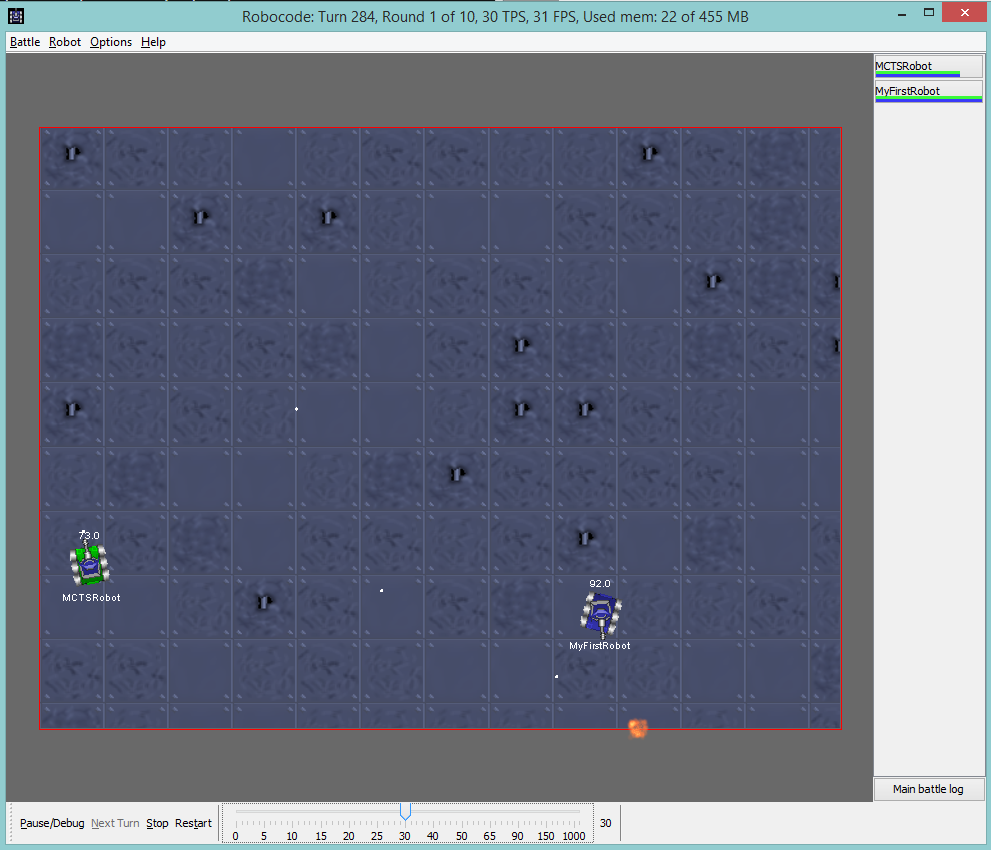
\includegraphics[width=\columnwidth]{Images/RobocodeBattle01}}
\caption{A battle between two robots..}
\label{figure--RobocodeBattle01}
\end{figure}

A robot starts with 100 energy, no idea of where the enemies are and can either move (ahead or back), turn its base, turn its gun, turn its radar or fire its gun during a turn. Moving and turning has no influence on the energy of the robot, but firing the gun and getting hit by bullets decrease the energy of the robot. When a robot is out of energy, it dies. There are limits to how much a robot can move or turn during a single turn\cite{wiki:robocodeGamePhysics}, as having no limits would break the game.

While a robot is limited to how much it can move or turn during a single turn, its API\cite{robocodeAPI} makes the process easier. For example, if a robot wants to move 100 pixels, it call the method Ahead(100). This method does not return until it has moved the chosen distance, and will thereby prevent other methods from being called meanwhile. As a robot can move no more than 8 pixels per turn, that is, best-case, $\frac{100}{8} = 12.5$ turns in which it only moves, something that is important to keep in mind when designing a robot.

In order to figure out where the enemy is, the robot needs to use its radar. The robot's radar is constantly active and scanning in in a straight line. If an enemy is detected by the radar, which can happen when the radar turns\footnote{The radar is connected to the gun, which is connected to the base of the robot. If one of those turn, the radar turns with them.}, the robot's OnScannedRobot() method is called, even if the robot is moving or turning already. When the method returns, the robot resumes doing what it was doing.

When the OnScannedRobot() method is called, it is possible to get some information about the scanned robot. The information is limited to the following: The enemy robot's heading, velocity and energy, the bearing our gun has and the distance to the enemy. This means that a robot will have to calculate the other robot's position in order to get that information, and that it is impossible to know where another robot's gun is pointing. Due to this, it is difficult to keep track of what an enemy robot is doing.

Firing the gun is a bit different from moving and turning. Firing the gun can be done with a power level between 1.0 and 3.0. The power level determines how much energy the robot loses (at a 1:1 ratio), but also determines the damage and velocity of the bullet. The more power, the more damage it deals if it hits and the slower the velocity is. Firing the gun also produces gun heat, and a robot is unable to fire as long as its gun is hot.

The rules and the API mean that it is possible to write a simple robot easily, but developing a good robot is a challenge.

%How does the game work that you are using? 
%Description of Robocode

\textbf{Why do you need AI in this game?}
% AI in robocode :D


\subsection{Influence of Robocode mechanics on MCTS}
\label{03_01}

Robocode is, without a doubt, a partially observable game. A robot only knows its own information and occasionally knows where an enemy robot is and where it is heading. There is no way to get any information about the general game state either, so information about where bullets are and where they are heading is also unavailable.

These factors mean that MCTS has very little information to work with, both during its simulation and its evaluation steps. This will be a challenge, as MCTS will have to make assumptions about where the enemy robot is (even after scanning it, it will quickly move to a new position) and how the enemy behaves in order to be able to simulate a playout and evaluate the results of a playout. If the assumptions are off by just a little, it will have a major impact on how well MCTS does.

% Discuss challenge of little - and possibly inccorect - knowledge of current gamestate
% Partially Observable Game

\section{Methods}
\label{04}
Our current implementation assumes that there is only one opponent in the game. The more opponents that are added to the game, the less precise the simulations of the game state will become.

\subsection{Monte-Carlo implementation}
\label{04_MCTS}

Our implementation of the MCTS algorithm differs from the original MCTS algorithms in a few of ways. The two most interesting differences are related to our child selection and our search depth.

\subsubsection{Child Selection}
When a node selects which child it should explore, normal MCTS chooses the child based on the UCT\cite{kocsis2006bandit} value of the children. It is possible, however, that a child will score lower than the average of its siblings when playout happens, thus leaving the child with a low UCT-value. As higher UCT values are prioritized by MCTS, the parent of the bad child will not be explored for quite some time (if ever again). This will generate an extremely asymmetric tree, which we would like to prevent. In order to do so, we only use the UCT value for exploration if all children of a the node we are exploring has been visited at least three times.

Through trial and error, we concluded that an exploration constant of 1 was what worked best in our implementation of Monte-Carlo Tree Search. In general, a higher exploration constant will lead to a more breadth-first search than a depth-first search, which is desirable for our current implementation as we do not have the luxury to simulate too far down the tree (both due to time constraints and due to inaccuracy in simulation).

\subsubsection{Max Search Depth}
Due to the nature of Robocode, we are unable to simulate our opponents properly (see section \ref{03}). This means that our simulations become more inaccurate the further down the tree we go. We chose to incorporate a maximum search depth to prevent simulations that were too inaccurate from affecting the tree too much. We chose a maximum search depth of 25, as it lets us reach a simulation that is relevant, without risking that the simulation becomes highly inaccurate.

\subsubsection{Branching Factor}
The branching factor of the algorithm is equal to the number of different moves that can be made by our robot in a single turn. This is a staggeringly high number, as the game uses double precision for degrees, distances, and firing power. Because of this, we have discretized the different options down to 32 (see equation \ref{eq_branchingfactor}).
\begin{equation}
\begin{split}
\label{eq_branchingfactor}
32 = 5 (speed intervals) + 11 (robot turn intervals)\\
+9 (gun turn intervals) + 5 (radar turn intervals) 
\\+ 2 (shoot)
\end{split}
\end{equation}
\subsection{Game Simulation}
Because Robocode is somewhat competitive - the inner workings of the game is not accessible from a robot - we had to do an emulation of the game in order to simulate future game states in the MCTS tree. Each node contains a game state which consists of information about our robot, the enemy robot, the projectiles that are currently flying through the air, and the instructions given to our robot in order to get from the previous game state to this one.

When simulating the next tick of the game, we follow steps 4 \& 5 of the Robocode Processing Loop\cite{wiki:robocodeGamePhysics}. Currently we do not simulate our robot and the enemy robot simultaneously, which is a difference between our simulation and the Robocode Processing Loop.
\subsubsection{Bullets} 
Our bullet simulation involves getting the next position of every currently active bullet and using those new positions to check for collisions with the two robots.
\subsubsection{Our Robot}
The Monte-Carlo Tree Search selects a robot instruction for the game state simulation to use when getting the next state of our robot. Currently we do not simulate collisions between robots (ramming) or radar scans.
\subsubsection{Enemy Robot}
When we simulate the enemy robot, we assume that it knows the location of all projectiles that are currently active. If the next position of the enemy robot is hit by a bullet, we assume that it will prioritize dodging this projectile. If it attempts to do so, it will search for another possible location that it can get to this turn that will not be hit by a projectile. In addition, we assume that the enemy knows our location and will attempt to turn its gun towards our robot. If the angle to our robot is within five degrees of the enemy gun, we assume that he will fire at our robot.

\subsection{Evaluation Heuristic}
When the Monte-Carlo Tree Search algorithm calls for the score of a node (game state), we use a heuristic (equation \ref{eq_heuristic_1}) to evaluate the state of the game at that node. 
\begin{equation}
\label{eq_heuristic_1}
score = OurRobotScore +  \left(\frac{1}{2} \frac{1}{100} EnemyEnergy\right)
\end{equation}
Equation \ref{eq_heuristic_2} describes how we calculate the score of our own robot.
\\Where \textit{EnergyScore} is $\left(\frac{1}{100}OurEnergy\right)$, \textit{BulletDamageScore} is the amount of damage dealt by bullets until this point, \textit{ShootScore} is 0.1 if we shot this round; 0.0 if not. \textit{MovementScore}\footnote{MovementScore is also penalized if the robot moves too close to the walls of the battlefield.} is the change in velocity that the robot made. If the robot did not change velocity or move, \textit{MovementScore} is instead given a $-1$ score. Finally the movement score is multiplied by $1.5$. \textit{RobotHeadingScore} is the amount of degrees that the robot turned this round multiplied by 0.4.
\begin{equation}
\begin{split}
\label{eq_heuristic_2}
ourRobotScore = EnergyScore+ShootScore\\
BulletDamageScore+MovementScore\\
+RobotHeadingScore
\end{split}
\end{equation}

\subsection{Interfacing it to the Game}
Because the main "gameplay" of Robocode is actually coding a robot, we simply coded the robot inside the framework provided to all Robocode players.

\section{Results}
\label{05}
In this section, we discuss how well different versions of our robot played against some sample robots provided with the Robocode installation. We also present data gathered while testing as well as evaluate the significant differences between each robot (if any).

\footnote{The variances were not equal between Default and MCTS-3, so a different critical t-value was used.}

\subsection{Test Set-Up}
We tested four different set-ups of the robot versus four different sample robots. Each test consisted of 10 tests of a 10-round battle with otherwise default Robocode rules. In order to test the effect of each setting, we only changed a single setting in each variation of our robot from our default robot. Because of the large number of different possible combination of settings, it is not likely that we have found the best possible one. The settings for our robots can be seen in table \ref{table-robotsettings}.

\subsubsection{Enemy Robots} 
We tested our robot against the \textit{MyFirstRobot}, \textit{SittingDuck}, \textit{Spinbot}, and \textit{Tracker} sample robots. \textit{MyFirstRobot} moves in a see-saw motion, rotates its gun and fires whenever it scans another robot. \textit{Spinbot} moves in a circular motion and fires a powerful shot whenever it scans an enemy. The \textit{Tracker} robot scans for a target, locks on to it, moves close and then fires at the target. As the name suggests, the \textit{SittingDuck} takes no action, does not move and does not react. It is often used to test how well the guns of a robot works.

We have not provided tables and data sets for the results of our tests versus the \textit{SittingDuck} robot, as we obtained a 100\% score against it with all four versions of the MCTS robot on every trial. 

\begin{table}
\begin{center}
\renewcommand{\arraystretch}{1}
\caption{Robot settings for score rewards}
\label{table-robotsettings}
\begin{tabular}{|c | c | c |c |}
\hline
Robot & Movement & Turning & Shooting\\
\hline
Default & 1.5 & 0.4 & 0.1\\
\hline
MCTS-1 & \textbf{3.0} & 0.4 & 0.1\\
\hline
MCTS-2 & 1.5 & \textbf{0.8} & 0.1\\
\hline
MCTS-3 & 1.5 & 0.4 & \textbf{0.2}\\
\hline
\end{tabular}
\end{center}
\end{table}

\subsubsection{Default-MCTS Robot}
We established the baseline "Default" robot settings by trying out different settings and deciding on a combination that seemed to be somewhat successful. The settings used for this robot offer a good compromise between shooting, moving, and turning. This default robot is somewhat trigger happy, however, and at times attempts to shoot every time it is possible.

\subsubsection{MCTS-1}
This robot should prioritize movement more than it ended up doing. It is, however, difficult to truly evaluate how much more it moves without tracking it specifically, which we did not. 

\subsubsection{MCTS-2} 
This robot is highly rewarded for turning around, which causes it to spin wildly while it shoots seemingly at random. It is possible that the doubling of the turning reward was too much and it would have been more useful to test with less of an increase (or perhaps even a decrease).

\subsubsection{MCTS-3}
We had anticipated that this robot would shoot more than the default robot, but we did not notice any apparent difference in the amount of shots fired. This is likely due to the trigger happiness of the default robot; if it already shoots as often as it can, then increasing the shooting reward is unlikely to make much of a difference.

\subsection{Data}
The scoring data in this section is represented as percentages of the total score in a single battle, e.g. our robot got 25\% of the total points and the enemy robot got the last 75\%. We represent it as such because of the stochastic nature of spawning positions and robot heading at the start of a round. By comparing percentage of the scores instead of absolute values, we are letting these random factors influence the results in the least possible way.

\subsubsection{Default-MCTS Robot}
As the default-MCTS robot was the baseline for our tests, we have done all significance comparisons using the test data for this robot.

Table \ref{table-default-score} indicates large differences in performance against the three different enemy robots. While the default robot never gets below 23\% score against \textit{MyFirstRobot}, it does poorly against the \textit{Spinbot} and even worse against the \textit{Tracker} robot. Interestingly, the robot is consistently poor against the \textit{Tracker} robot, as evidenced by the lower standard deviation (and seen on figure \ref{figure-BarGraph}\footnote{The variance bars on the graph represent standard deviation.}).

The distribution of scores against the enemy robots are shown in figures \ref{figure--Distribution-MFR}, \ref{figure--Distribution-Spinbot}, and \ref{figure--Distribution-Tracker}. The values are the decimal representations of the percentage scores achieved by the default robot. While the scores mostly fit somewhat nicely around the bell curve, the results against both \textit{MyFirstRobot} and \textit{Spinbot} have one rather extreme outlier.

\begin{table}
\begin{center}
\renewcommand{\arraystretch}{1.3}
\caption{Score for the Default-MCTS Robot}
\label{table-default-score}
\begin{tabular}{|c | c | c |c | c| c |}
\hline
Enemy & Mean & Median & Mode & Std. Dev & Std. Err.\\
\hline
MyFirstRobot & 25.6\% & 25.4\% & None & 1.609 & 0.509\\
\hline
Spinbot & 15.7\% & 16.3\% & None & 2.145 & 0.678 \\
\hline
Tracker & 10.8\% & 10.5\% & None & 0.779 & 0.246 \\
\hline
\end{tabular}
\end{center}
\end{table}

\begin{figure}[htp]
\centerline{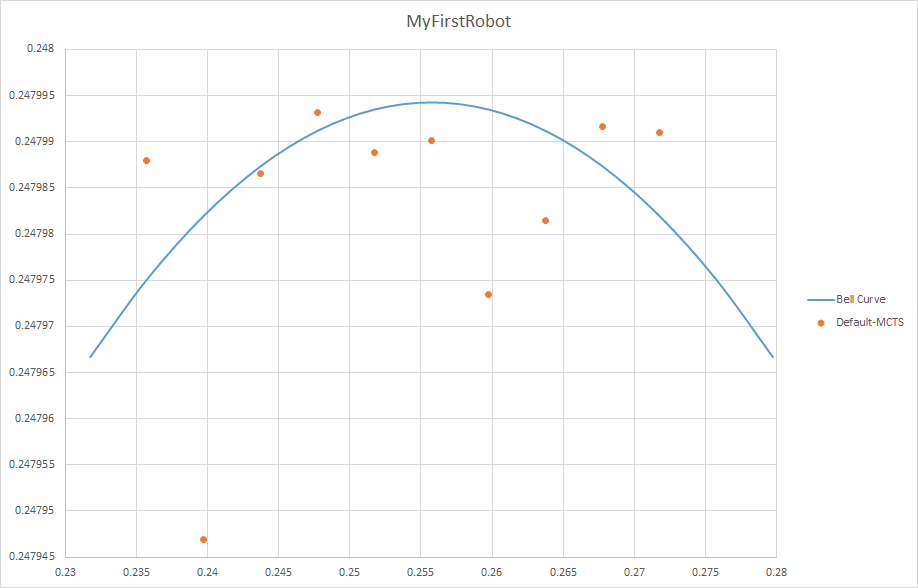
\includegraphics[width=\columnwidth]{Images/MyFirstRobotDistribution}}
\caption{Distribution of results by default-MCTS against the "MyFirstRobot".}
\label{figure--Distribution-MFR}
\end{figure}

\begin{figure}[htp]
\centerline{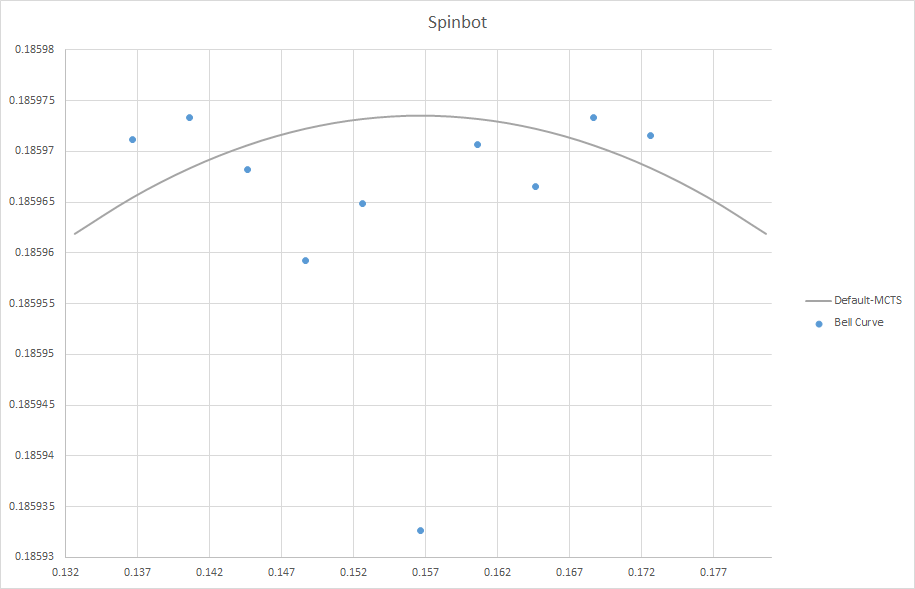
\includegraphics[width=\columnwidth]{Images/SpinbotDistribution}}
\caption{Distribution of results by default-MCTS against the "Spinbot" robot.}
\label{figure--Distribution-Spinbot}
\end{figure}

\begin{figure}[htp]
\centerline{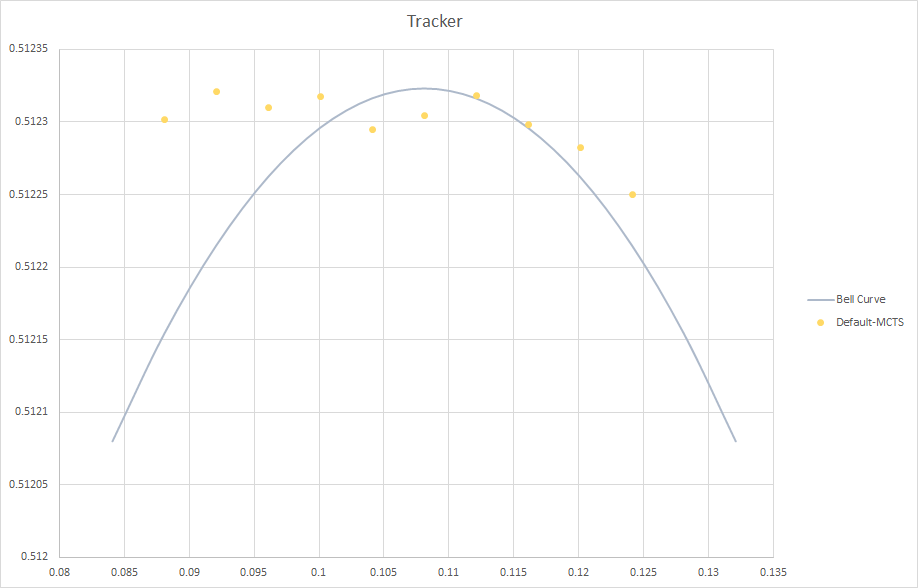
\includegraphics[width=\columnwidth]{Images/TrackerDistribution}}
\caption{Distribution of results by default-MCTS against the "Tracker" robot.}
\label{figure--Distribution-Tracker}
\end{figure}

\begin{figure}[htp]
\centerline{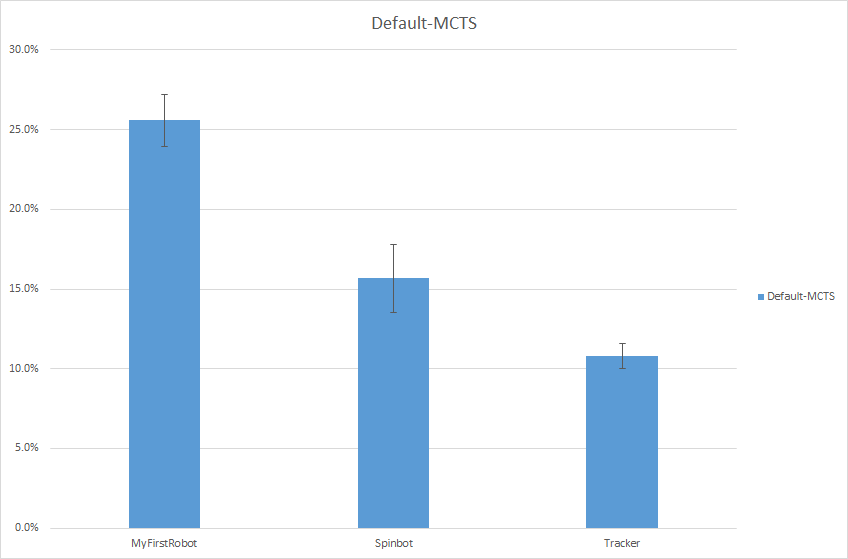
\includegraphics[width=\columnwidth]{Images/BarGraph}}
\caption{Mean score percentages for the Default MCTS controller.}
\label{figure-BarGraph}
\end{figure}

\subsubsection{Other versions}
Tables \ref{table-MCTS1-score}, \ref{table-MCTS2-score}, and \ref{table-MCTS3-score} show the scores of the three variations of our robot. When compared to the default-MCTS robot, the only robot variation that showed a significant difference was the MCTS-2 robot, which was expected with the observed behaviour described previously.

\begin{table}
\begin{center}
\renewcommand{\arraystretch}{1.3}
\caption{Score for the MCTS-1 Robot}
\label{table-MCTS1-score}
\begin{tabular}{|c | c | c |c | c| c |}
\hline
Enemy & Mean & Median & Mode & Std. Dev & Std. Err.\\
\hline
MyFirstRobot & 27.2\% & 26.6\% & None & 3.292 & 1.041\\
\hline
Spinbot & 19.5\% & 19.3\% & None & 2.437 & 0.771 \\
\hline
Tracker & 13.7\% & 13.9\% & 14.3 & 1.789 & 0.567 \\
\hline
\end{tabular}
\end{center}
\end{table}

\begin{table}
\begin{center}
\renewcommand{\arraystretch}{1.3}
\caption{Score for the MCTS-2 Robot}
\label{table-MCTS2-score}
\begin{tabular}{|c | c | c |c | c| c |}
\hline
Enemy & Mean & Median & Mode & Std. Dev & Std. Err.\\
\hline
MyFirstRobot & 8.4\% & 8.3\% & None & 1.854 & 0.586\\
\hline
Spinbot & 3.4\% & 3.6\% & 3.7 & 0.970 & 0.307  \\
\hline
Tracker & 4.4\% & 4.5\% & 4.6 & 0.491 & 0.155 \\
\hline
\end{tabular}
\end{center}
\end{table}

\begin{table}
\begin{center}
\renewcommand{\arraystretch}{1.3}
\caption{Score for the MCTS-3 Robot}
\label{table-MCTS3-score}
\begin{tabular}{|c | c | c |c | c| c |}
\hline
Enemy & Mean & Median & Mode & Std. Dev & Std. Err.\\
\hline
MyFirstRobot & 26.0\% & 25.8\% & None & 3.054 & 0.965\\
\hline
Spinbot & 15.9\% & 15.1\% & None & 3.319 & 1.049  \\
\hline
Tracker & 11.4\% & 11.1\% & None & 1.303 & 0.413 \\
\hline
\end{tabular}
\end{center}
\end{table}

\subsection{Evaluation}

%which robot was best
\subsubsection{Speed}
The speed of the algorithm is capped at 10 milliseconds per iteration in order to avoid skipping any turns in robot. This does not allow the algorithm to search very deep into the tree, but we believe this to be a somewhat positive behaviour. Because the simulation of the game state and the assumptions we make about the actions taken by the opponent can potentially be wildly inaccurate, we will rarely benefit from simulating too far into the future.

\begin{table}
\begin{center}
\renewcommand{\arraystretch}{1}
\caption{Significance test using the MyFirstRobot Robot}
\label{table-MFS-significance}
\begin{tabular}{|c | c | c |c | c | c |}
\hline
Controller & Mean & Variance & t-value & critical t & Significant\\
\hline
Default & 0.256 & 0.00025 & N/A & N/A & N/A\\
\hline
MCTS-1 & 0.272 & 0.00108 & 1.397 & 2.101 & No\\
\hline
MCTS-2 & 0.844 & 0.00034 & -22.067 & 2.101 & Yes\\
\hline
MCTS-3 & 0.260 & 0.0009 & 0.354 & 2.145 & No\\
\hline
\end{tabular}
\end{center}
\end{table}




\section{Conclusions}
\label{06}
The conclusion goes here.

What are the strengths and shortcomings of your method? Why did you choose method X instead of Y? How well would it generalize to other game genres? How would you develop it further, if you had time?

%\section*{Appendix}
Put your appendix here if you have any.

%Bibliography
\begin{filecontents*}{\jobname.bib}

@article{gelly2011monte,
	title		= {{M}onte-{C}arlo tree search and rapid action value estimation in computer {G}o},
	author	= {Gelly, Sylvain and Silver, David},
	journal	= {Artificial Intelligence},
	volume	= {175},
	number	= {11},
	pages		= {1856--1875},
	year		= {2011},
	publisher	= {Elsevier},
	url 		= {http://www.sciencedirect.com/science/article/pii/S000437021100052X},
	note		= {[Online; accessed \today]}
}

@article{browne2012survey,
	title 		= {{A} survey of monte carlo tree search methods},
	author 	= {Browne, Cameron B and Powley, Edward and Whitehouse, Daniel and Lucas, Simon M and Cowling, Peter I and Rohlfshagen, Philipp and Tavener, Stephen and Perez, Diego and Samothrakis, Spyridon and Colton, Simon},
	journal 	= {Computational Intelligence and AI in Games, IEEE Transactions on},
	volume 	= {4},
	number 	= {1},
	pages 	= {1--43},
	year 		= {2012},
	publisher 	= {IEEE},
	url 		= {http://ieeexplore.ieee.org/xpls/abs\_all.jsp?arnumber=6145622},
	note		= {[Online; accessed \today]}
}

@phdthesis{chaslot2010monte,
	title		= {Monte-carlo tree search},
	author	= {Chaslot, Guillaume},
	year		= {2010},
	school		= {PhD thesis, Maastricht University},
	url 		= {https://project.dke.maastrichtuniversity.nl/games/files /phd/Chaslot\_thesis.pdf},
	note		= {[Online; accessed \today]}
}

@incollection{auger2011multiple,
	title		= {{M}ultiple tree for partially observable {M}onte-{C}arlo tree search},
	author	= {Auger, David},
	booktitle	= {Applications of Evolutionary Computation},
	pages		= {53--62},
	year		= {2011},
	publisher	= {Springer},
	url 		= {http://link.springer.com/chapter/10.1007/978-3-642-20525-5\_6},
	note		= {[Online; accessed \today]}
}

@inproceedings{silver2010monte,
	title		= {{M}onte-{C}arlo planning in large {POMDP}s},
	author		= {Silver, David and Veness, Joel},
	booktitle	= {Advances in Neural Information Processing Systems},
	pages		= {2164--2172},
	year		= {2010},
	url 		= {http://papers.nips.cc/paper/4031-monte-carlo-planning-in-large-pomdps},
	note		= {[Online; accessed \today]}
}

@inproceedings{thrun1999monte,
	title		= {{M}onte {C}arlo {POMDP}s.},
	author	= {Thrun, Sebastian},
	booktitle	= {NIPS},
	volume	= {12},
	pages		= {1064--1070},
	year		= {1999},
	url 		= {ftp://ftp.irisa.fr/local/as/campillo/micr/bib/thrun1999b.pdf},
	note		= {[Online; accessed \today]}
}

@inproceedings{pepels2012enhancements,
	title		= {{E}nhancements for {M}onte-{C}arlo tree search in {M}s {P}ac-{M}an}},
	author	= {Pepels, Tom and Winands, Mark HM},
	booktitle	= {Computational Intelligence and Games (CIG), 2012 IEEE Conference on},
	pages		= {265--272},
	year		= {2012},
	organization	= {IEEE},
	url 		= {http://ieeexplore.ieee.org/xpls/abs\_all.jsp?arnumber=6374165\&tag=1},
	note		= {[Online; accessed \today]}
}

@incollection{kocsis2006bandit,
	title		= {{B}andit based {M}onte-{C}arlo planning},
	author	= {Kocsis, Levente and Szepesv{\'a}ri, Csaba},
	booktitle	= {Machine Learning: ECML 2006},
	pages		= {282--293},
	year		= {2006},
	publisher	= {Springer},
	url 		= {http://link.springer.com/chapter/10.1007/11871842\_29},
	note		= {[Online; accessed \today]}
}


@misc{robocode,
	title		= {Robocode},
	author	= {Nelson, Matthew A. and Larsen, Flemming N.},
	year		= {2001},
	url 		= {http://robocode.sourceforge.net/},
	note		= {[Online; accessed \today]}
}

@misc{robocodeAPI,
	title		= {Robocode API},
	author	= {Nelson, Matthew A. and Robocode contributers},
	year		= {2014},
	url 		= {http://robocode.sourceforge.net/docs/robocode.dotnet/Index.html},
	note		= {[Online; accessed \today]}
}

@misc{wiki:robocodeGamePhysics,
	title		= {Game Physics},
	author	= {Robocode Wiki},
	year		= {2007},
	url 		= {http://robowiki.net/wiki/Robocode/Game\_Physics},
	note		= {[Online; accessed \today]}
}


@misc{mctsai,
	title 		= {mcts.ai},
	author 	= {Cameron Browne},
	url 		= {http://mcts.ai/about/index.html},
	note		= {Accessed \today}
}

@techreport{pinto2002introducing,
  title={Introducing the min--max algorithm},
  author={Pinto, Paulo},
  year={2002},
  institution={Tech. rep., AI Depot}
}

\end{filecontents*}

\bibliographystyle{IEEEtran}
%\nocite{*}
\bibliography{\jobname}

% That's all folks...
\end{document}
